%%%%%%%%%%%%%%%%%%%%%%%%%%%%%%%%%%%%%%%%%%%%%%%%%%%%%%%%%%%%%%%%%%%%%%%%%%%%%%%%%%%%
%%----------------------------------------------------------------------------------
% DO NOT Change this is the required setting A4 page, 11pt, onside print, book style
%%----------------------------------------------------------------------------------
\documentclass[a4paper,11pt,oneside]{book} 
\usepackage{style} % DO NOT REMOVE THIS LINE. 
%%%%%%%%%%%%%%%%%%%%%%%%%%%%%%%%%%%%%%%%%%%%%%%%%%%%%%%%%%%%%%%%%%%%%%%%%%%%%%%%%%%%


%%%%%%%%%%%%%%%%%%%%%%%%%%%%%%%%%%%%%%%%%%%%%%%%%%%%%%%%%%%%%%%%%%%%%%%%%%%%%%%%%%%%
\begin{document}

    \captionsetup[figure]{margin=1.5cm,font=small,name={Figuur},labelsep=colon}
    \captionsetup[table]{margin=1.5cm,font=small,name={Tabel},labelsep=colon}
    
    \frontmatter
    
    %%%%%%%%%%%%%%%%%%%%%%%%%%%%%%%%%%%%%%%%%%%%%%%%%%%%%%%%%%%%%%%%%%%%%%%%%%%%%%%%
    \begin{titlepage}      
        \begin{center}
            
\includegraphics[width=9cm]{figures/LogoFaculteit.png}\\[0.5cm]
            {\LARGE Universiteit Antwerpen\\[0.5cm]
            Faculteit Toegepaste\\ Ingenieurswetenschappen}\\[2cm]
			%{\color{blue} \rule{\textwidth}{1pt}}
			
			% -------------------------------
			% You need to edit some details here
			% -------------------------------  
            \linespread{1.2}\huge {
                %%%%%%%%%%%%%%%%%%%%%%%%%%%%
                %TODO: 1 TITLE of Your PROJECT 
                %%%%%%%%%%%%%%%%%%%%%%%%%%%%
                % change the following line                
                Ontwerp en ontwikkeling van een modulair elektronisch pipetteersysteem
            
            }
            \linespread{1}~\\[2cm]
			%{\color{blue} \rule{\textwidth}{1pt}}
            {\Large 
                %%%%%%%%%%%%%%%%%%%%%%%%%%%%
                %TODO: 2 YOUR NAME
                %%%%%%%%%%%%%%%%%%%%%%%%%%%%             
                % change the following line
                Sybe De Backer
                % change end             
            }\\[1cm] 
            

            {\large 
                %%%%%%%%%%%%%%%%%%%%%%%%%%%%
                %TODO: 3 YOUR NAME Supervisor's name(s)
                %%%%%%%%%%%%%%%%%%%%%%%%%%%%             
                % change the following line                
                \emph{Promotor:} Prof.\ Dr.\ Ir. Amélie Chevalier\\
                \emph{Mentor:} Dr.\ Ing.\ Jona Gladines}\\[1cm] % if applicable
            
    		% PLEASE DO NOT CHANGE THIS TEXT %
            \large Een eindwerk ingediend bij\\Universiteit Antwerpen voor het diploma\\
            %%%
            %TODO:  verify your degree name
            \textit{Bachelor in de Industriële Wetenschappen: Elektromechanica}\\[0.3cm]
            %% 
            %TODO:  verify your degree in
            \vfill
            
            \textit{Academiejaar 2024--2025 \\[0.3cm]}
            %\today % Please update this date you can use \date{April 2020} for fixed date
        \end{center}
    \end{titlepage}
    
    
    % -------------------------------------------------------------------
    % Declaration
    % -------------------------------------------------------------------
    %\newpage
    \thispagestyle{empty}
    \chapter*{\Large Declaration}
    % PLEASE CHANGE THIS TEXT EXCEPT YOUR NAME%
    % -------------------------------
    %TODO: PLEASE ONLY UPDATE HERE -- PLEASE WRITE YOUR NAME %    
    % ------------------------------- 
    Ik,
    %%%%%%%%%%%%%%%%%%%%%%%
     Sybe De Backer, % Madatory part  TODO
    %%%%%%%%%%%%%%%%%%%%%%%
    bevestig ik dat dit mijn eigen werk is en dat de cijfers, tabellen, vergelijkingen, stukjes code, kunstwerken en illustraties in dit rapport origineel zijn en niet zijn overgenomen uit het werk van anderen, behalve wanneer het werk van anderen expliciet is erkend, geciteerd en waarnaar wordt verwezen. Ik begrijp dat als ik dit niet doe, dit zal worden beschouwd als een geval van plagiaat. Plagiaat is een vorm van academisch wangedrag en zal dienovereenkomstig worden bestraft. \\
    
    \begin{flushright}
	%------------------------------ 
	% change the following line
    %TODO: PLEASE UPDATE  Your Name  -------------------------------%
	Sybe De Backer % Please change it to your name
    
    \today
    \end{flushright}

     
    % -------------------------------------------------------------------
    % Abstract and Acknowledgement
    % -------------------------------------------------------------------
    
    %\chapter{abstract}
    % -------------------------------------------------------------------
	% Acknowledgement
	% -------------------------------------------------------------------
       
    % -------------------------------------------------------------------
    % Contents, list of figures, list of tables
    % -------------------------------------------------------------------
    
    \tableofcontents
    \listoffigures
    \listoftables
    \input{glossaries} %  Enter your list of Abbreviation and Symbols in this file



    
    
    %%%%%%%%%%%%%%%%%%%%%%%%%%%%%%%%%%%%%%%%%%%%%%%%%%%%%%%%%%%%%%%%%%%%%%%%
    %%                                                                    %%  
    %%  Main chapters and sections of your project                        %%  
    %%  Everything from here on needs updates in your own words and works %%
    %%                                                                    %%
    %%%%%%%%%%%%%%%%%%%%%%%%%%%%%%%%%%%%%%%%%%%%%%%%%%%%%%%%%%%%%%%%%%%%%%%%
    \mainmatter
    % Read for preparation of document in LaTex 
    % Lamport, L. (1986), LATEX: A Document Preparation System, Addison-Wesley.
    
    \chapter{Inleiding}
\section{laboratorium-automatisatie}
In de afgelopen jaren hebben robotische processen de manier waarop we experimenten en de bijhorende labotaken uitvoeren, veranderd. Geautomatiseerde systemen hebben, vooral in biomedisch en moleculair onderzoek, een enorm potentieel aangetoond voor het verhogen van de reproduceerbaarheid van experimenten, het stroomlijnen van experimentele methoden en het verminderen van de impact van menselijke fouten.\cite{RN5} 
\\[12pt]Deze thesis zal zich richten op de ontwikkeling van een robotisch pipetteersysteem dat is afgestemd op de behoeften van de onderzoeksgroep ``Translational Neurosciences'' aan de Universiteit Antwerpen. Het doel van dit onderzoek is om de robuustheid en reproduceerbaarheid van hun experimenten te verbeteren. Dit gebeurt in het kader van een bredere automatisering van hun laboratorium. Door één van de kernuitdagingen in experimentele reproduceerbaarheid, namelijk het maken van menselijke fouten bij repetitief werk, aan te pakken probeert dit werk bij te dragen om betrouwbare onderzoeksinstrumenten te creëren.

\section{Breder kader}

\subsection{Reproduceerbaarheidscrisis}
Reproduceerbaarheid is een hoeksteen van wetenschappelijk onderzoek en zorgt ervoor dat resultaten onafhankelijk kunnen worden geverifieerd. Studies hebben echter gewezen op een groeiende reproduceerbaarheidscrisis in onder meer biomedisch onderzoek, veroorzaakt door inconsistenties in handmatige procedures, subjectieve beoordelingen en omgevingsvariabiliteit.\ \cite{RN2} De reproduceerbaarheidscrisis verwijst naar de moeilijkheid om wetenschappelijke resultaten consistent te reproduceren, een probleem dat zowel technische als menselijke oorzaken kent. 
\\[12pt]Vaak wordt er gekeken naar de sociale en economische aspecten van wetenschap.\cite{RN12} De druk om origineel onderzoek te publiceren is zo groot dat dit een druk uitoefent op de bestaande systemen van peer-evaluatie en soms worden resultaten herwerkt tot ze een significante ontdekking vertonen met methodes als “p-hacking”.\cite{RN2,RN6} Er zijn echter ook technische beperkingen. Zo worden door menselijke fouten handelingen niet altijd uitgevoerd zoals ze in het experiment beschreven staan. 
\\[12pt]Dit gebrek aan succesvolle reproductie heeft een significante impact op bijvoorbeeld kankeronderzoek en andere gerelateerde onderzoeksdisciplines.\ \cite{RN4}

\section{Robotic labs als oplossing voor reproduceerbaarheidscrisis}
Door het automatiseren van enkele of alle taken wordt de mogelijkheid tot menselijke fout verminderd. Robots kunnen ervoor zorgen dat repetitieve taken telkens op dezelfde manier worden uitgevoerd. Bij het manueel pipetteren kunnen deze taken door vermoeidheid en fysieke klachten voor variatie zorgen.\ \cite{RN9} Doordat liquid handling robots programmeerbaar zijn en deterministisch werken is het mogelijk om de exacte handelingen uit te voeren zonder het risico dat stappen worden weggelaten.

\section{Probleemstelling}
Als einddoel zal er getracht worden om een systeem te ontwikkelen dat (met een API) zal toelaten om programmatisch pipethandelingen uit te voeren. Het systeem zal zo ontworpen worden dat het geïntegreerd kan worden met bestaande robots, als end effector. Door deze zo kostenefficiënt mogelijk te ontwerpen is het de bedoeling dat deze robot toegankelijk zal zijn voor laboratoria die de hoge investeringskosten van deze automatiseringssystemen willen vermijden. De thesis zal zich specifiek richten op het beantwoorden van volgende onderzoeksvraag:\begin{quote}
    \begin{center}
        \textbf{\textit{Welke ontwerp- en implementatievereisten zijn nodig voor de ontwikkeling van een programmeerbare, kostenefficiënte pipetrobot die reproduceerbaarheid in laboratoria verbetert?}}
    \end{center}
\end{quote}
Door een aanpasbaar en modulair ontwerp aan te bieden, kunnen laboratoria kiezen voor een oplossing die voldoet aan hun specifieke behoeften zonder overbodige kosten. Dit betekent ook dat er reeds bestaande software en hardware kunnen gebruikt worden om enerzijds de initiële kosten te drukken, en eveneens flexibiliteit en uitbreidbaarheid te bieden. Dit biedt een aantrekkelijk alternatief voor de dure commerciële systemen die vaak voorgeconfigureerd zijn en weinig ruimte laten voor aanpassing.
    \chapter{Achtergrond}


\section{Pipetteconcepten}
\subsection{Air-Displacement}
%\subsubsection{Eerste pipetten}
%Mondpipetten waren doorheen de 19e en in het begin van de 20e eeuw de standaard voor het pipetteren. In \cite{RN21} wordt bijvoorbeeld een ontwerp voor een mondpipet voorgesteld om steriliteitstesten mee uit te voeren. In 1950 werd door A. J. Swallow in\cite{RN18} de eerste mechanische pipet voorgesteld voor het pipetteren van radioactieve stoffen. Hierdoor was er geen contact mogelijk tussen de mond en de te pipetteren vloeistof. Dit helpt ook bij het vermijden van besmetting van labopersoneel zoals beschreven in \cite{RN20}.
\subsubsection{Theoretische achtergrond}
In\ \cite{RN15} staat beschreven hoe een air-displacement pipet werkt via de ideale gaswet. Er wordt een omgeving van lagere druk gecreëerd door het veranderen van het volume van de pipet voor aspiratie. Dit volume wordt ingenomen door de vloeistof waar de pipet zich in bevindt. Bij een mondpipet wordt deze negatieve druk gecreëerd door de longen van de operator. Bij de mechanische pipet wordt deze via de peer gecreëerd door deze initieel in te drukken en daarna terug te laten opvullen.
\subsubsection{Analoge pipetten}
Analoge pipetten, zoals beschreven in o.a.\ de patenten\ \cite{RN16} en\ \cite{RN17}, werken op basis van een zuigerwerking. De slag van de zuiger kan voor de aspiratie bepaald worden door middel van een wiel in geval van\ \cite{RN17} of door twee elementen in elkaar te schroeven in geval van\ \cite{RN16}. Bij\ \cite{RN17} zal dit wiel, door het axiaal verschuiven van een loodschroef, de zuigerstang verschuiven. In rustpositie zal deze dus korter lijken bij een kleiner ingesteld volume. De zuigerstang kan dan ingedrukt worden tot een stop-nut, deze blijft altijd op de zelfde plaats. Doordat de beginpositie aangepast wordt, wordt ook de slag van de zuiger aangepast. Hiermee wordt het volume bepaald.\ \cite{RN16} volgt een gelijkaardig principe. Hier zal echter de eindpositie bepaald worden door het onderste deel verder te schroeven. De analoge pipetten beschreven in deze patenten gebruiken air-displacement. In geval van\ \cite{RN17} gebeurt dit met een zuiger (44) die relatief verder van de pipetteer-punt (28) staat dan bij\ \cite{RN16}.\ \cite{RN16} is eenvoudiger uitgevoerd dan\ \cite{RN17}. Er zijn minder dichtingen en er is geen display om het gewenste volume van af te lezen. Dit maakt echter ook dat\ \cite{RN16} meer problemen zal hebben op vlak van lekkage en dus precisie.

\subsection{Positive Displacement} % https://guides.library.bloomu.edu/litreview
    \chapter{Methode}
In dit hoofdstuk wordt het ontwerp en de realisatie van de ontworpen pipet besproken. Hierbij worden de verschillende onderdelen behandeld, als ook de gemaakte keuzes.

\section{Conceptueel ontwerp}
\subsection{Literatuurstudie}
De Literatuurstudie bestond voor een groot deel uit het bestuderen van beschikbare patenten. Patenten zoals\ \cite{RN16} en\ \cite{RN17} beschrijven analoge pipetten. Deze worden nog manueel bediend en hebben een relatief eenvoudige werking. Deze patenten waren belangrijk om de basiswerking van moderne pipetten te begrijpen. Ze tonen namelijk aan dat deze pipetten met één eenvoudige zuigerwerking werken. Dit is een belangrijke stap bij het ontwerp van de automatische pipet.
\\\textit{Zie \autoref{sec: Analoge pipetten} voor verdere toelichting betreffende de werking.}
\\[12pt]Verder werden de patenten \ \cite{RN35},\ \cite{RN36} en\ \cite{RN38} bestudeerd. Deze patenten beschrijven de werking van een, motorisch aangedreven, elektronische pipet. In het geval van\ \cite{RN36} en\ \cite{RN38} wordt niet toegelicht welk type motor gebruikt wordt. In het geval van\ \cite{RN35} wordt er vermeld dat er voor een stappermotor is gekozen. Deze patenten tonen aan dat de zuigerwerking van een pipet met een stappermotor kan gebeuren en dat deze met een hoge precisie kunnen werken. Ook dit is een belangrijke stap in het ontwerp van de automatische pipet.

\section{Hardware ontwerp}
Dit onderdeel behandelt de keuzes betreffende de hardware in dit project. De onderdelen die ge-3D-print zijn werden ontworpen in Autodesk Inventor en geprint met Prusa Mk3S en Mk4 printers.

\subsection{Muurelementen}
Zoals eerder vernoemd is voor het hardware ontwerp gekozen voor een modulaire oplossing. Dit laat toe om de verschillende onderdelen onafhankelijk van elkaar te ontwikkelen en indien nodig aan te passen. Dit maakt het in de toekomst ook mogelijk om dit ontwerp uit te breiden tot bijvoorbeeld een meerkanaals systeem. De verschillende modules worden geplaatst over geleidestaven, zoals in\ \autoref{fig:geleidestaven} te zien is. Deze geleidestaven zorgen ervoor dat de verschillende modules correct uitgeleind en geplaatst worden.
\\[12pt]De eerste ontwerpiteraties focusten zich hoofdzakelijk op het ontwerp van de muren. Deze zijn in PLA geprint. Aangezien de muren weinig structurele lasten moeten dragen is PLA een geschikte keuze. In de latere iteraties zijn de muren verdund en zijn de vlakken verdwenen zoals in \autoref{fig:hollowwalls} te zien is. Dit maakt de muren lichter en goedkoper. De muren zijn ook in verschillende hoogtes ontworpen met een geparametriseerd model. 
\\[12pt]Het afgeleverde model bestaat uit twee muurelementen van 40mm en een muurelement van 30mm. De twee elementen van 40mm voorzien ruimte voor de slag van de zuiger. Het muurelement van 30mm voorziet ruimte voor de askoppeling.
\\[12pt]\begin{minipage}[t]{0.49\textwidth}
    \vspace{0pt}
    \begin{figure}[H]
        \centering
        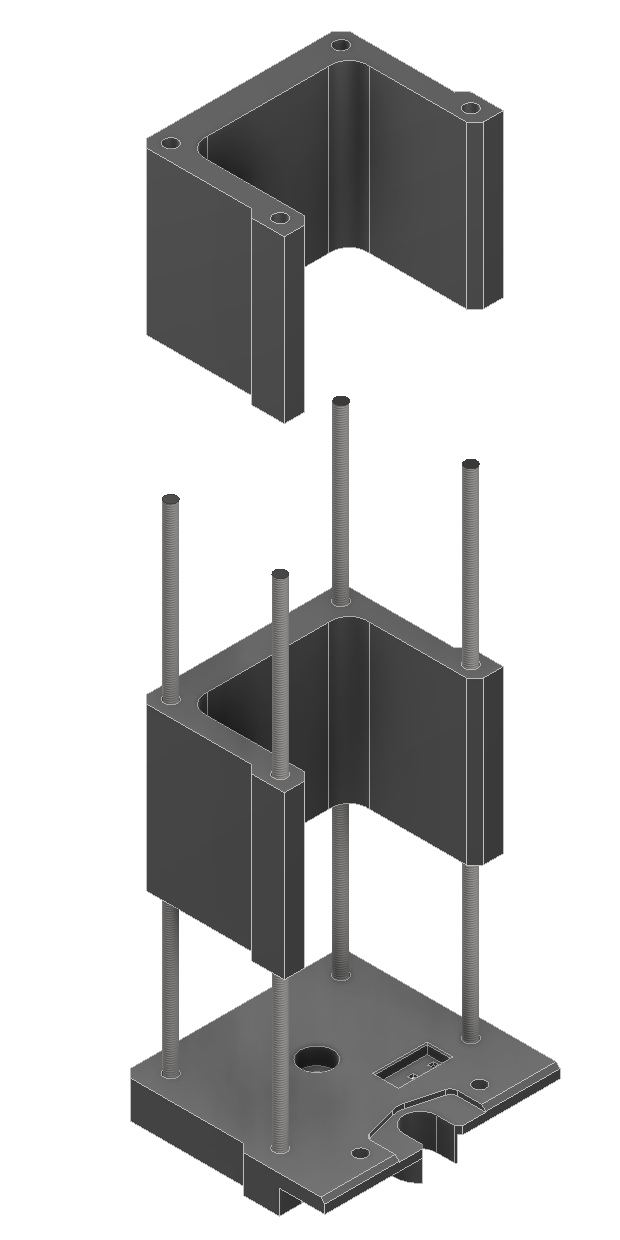
\includegraphics[height=6cm]{figures/GuidesDemonstration.png}
        \caption{Demonstratie van de geleidestaven.}\label{fig:geleidestaven}
    \end{figure}
\end{minipage}
\begin{minipage}[t]{0.49\textwidth}
    \vspace{0pt}
    \begin{figure}[H]
        \centering
        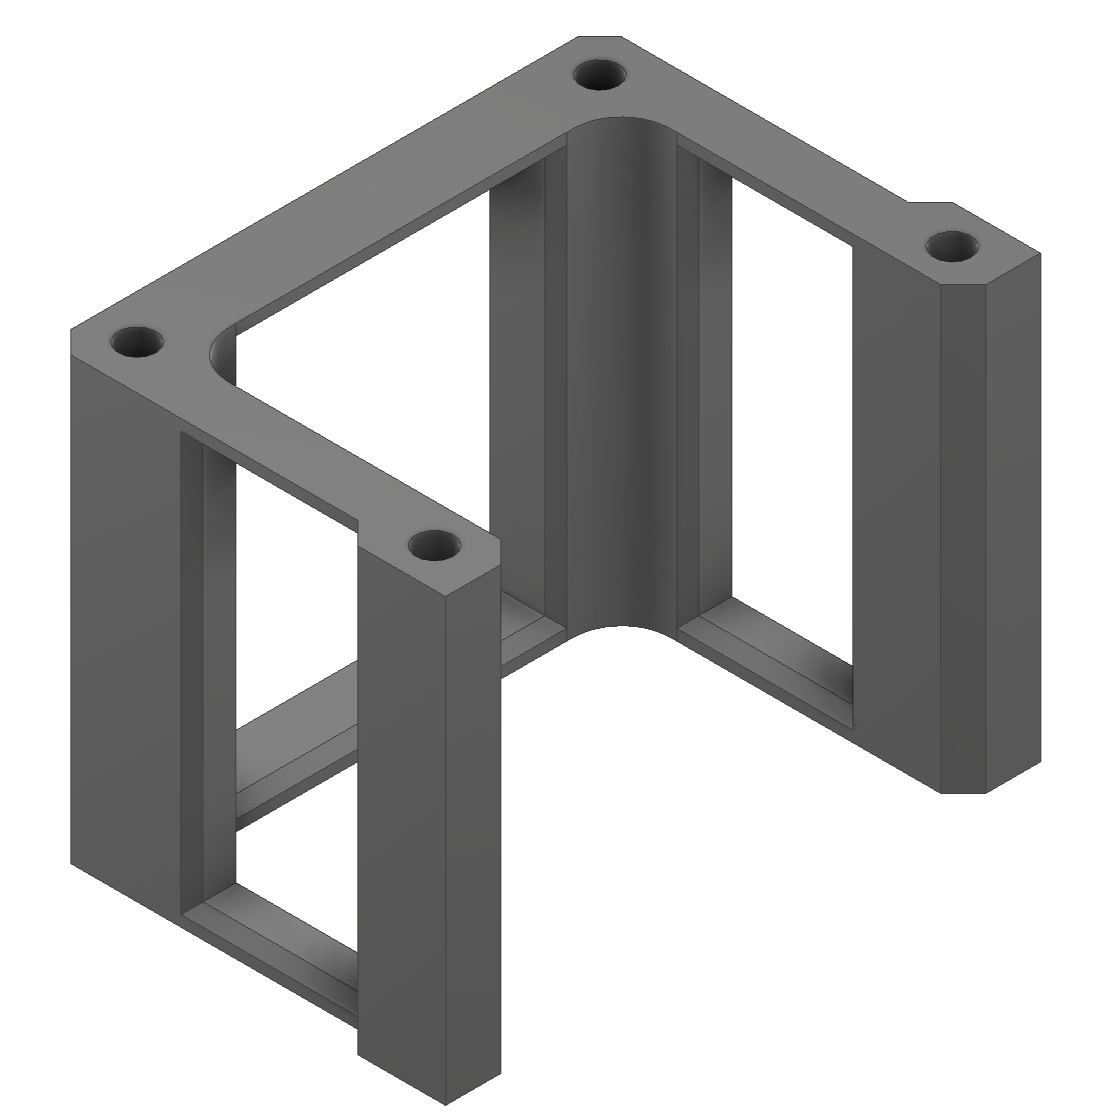
\includegraphics[height=6cm]{figures/Walls_1_w.png}
        \caption{Lichtere muren.}\label{fig:hollowwalls}
    \end{figure}
\end{minipage}\\

\subsection{Bodemplaat en geleidestaven}
De muurelementen en geleidestaven worden op de bodemplaat gemonteerd. De bodemplaat is hiervoor voorzien van gaten waar de geleidestaven doorheen kunnen. Onderaan de geleidestaven bevinden zicht twee tegengedraaide schroeven. Dit wordt bijvoorbeeld toegepast bij de montage van verkeerslichten zoals te zien in \autoref{fig:verkeerslichten}. Dit is een effectieve oplossing die gebruikt kan worden om ge-3D-printte elementen extra te versterken, alsook om de elementen in kleinere onderdelen te bevestigen en daarna aan te spannen. Zo wordt het in\ \cite{RN40} meerdere keren gebruikt.
\\[12pt]De tegengedraaide moeren (type ISO 4032-M3) passen in hiervoor voorziene gaten zoals te zien is in\ \autoref{fig:counterrotated}. Deze gaten bestaan uit twee trappen. De onderste trap heeft een zeshoekigevorm, gebaseerd op de afmetingen van de moer. De moer past net in dit gat maar kan slechts zeer weinig roteren. De tweede moer staat hier dan sterk tegenaan gedraaid zodat deze ook niet zal roteren. De twee trap van het gat is een cilindrisch gat waarin de moer vrij kan roteren. Deze rotatie is echter niet wenselijk, het gat is enkel voorzien zodat de eerste moer, ogeacht de oriëntatie van de tweede moer, in het hexagonale gat kan worden ingebracht.
\\[12pt]\\[12pt]\begin{minipage}[t]{0.49\textwidth}
    \vspace{0pt}
    \begin{figure}[H]
        \centering
        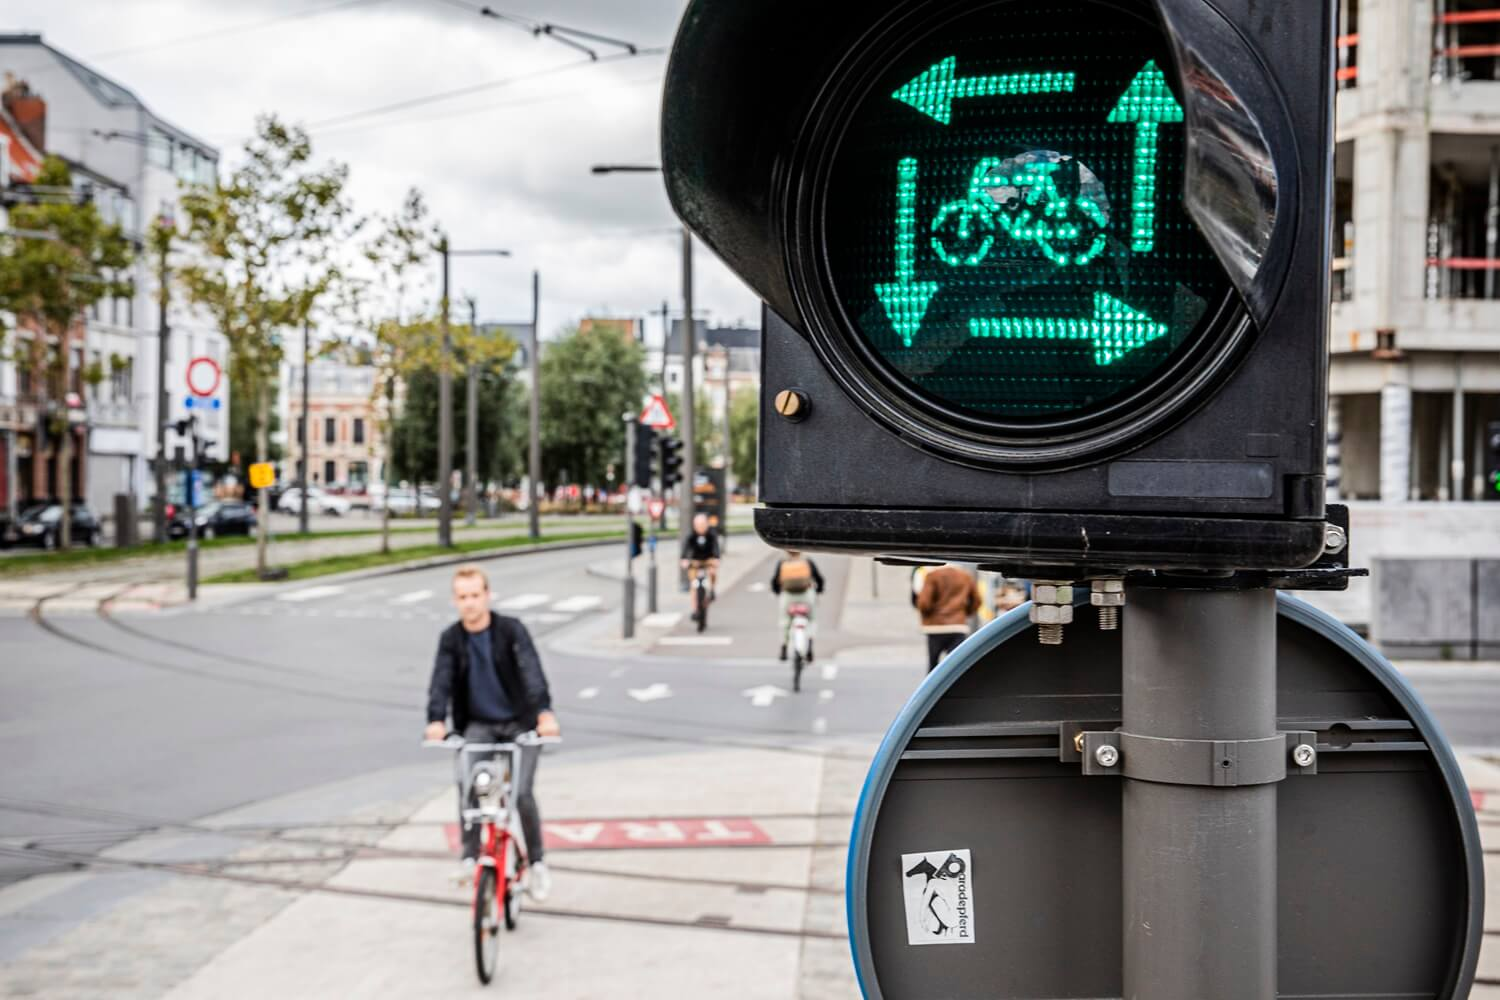
\includegraphics[height=4cm]{figures/verkeerssituaties48.jpg}
        \caption{Montage van verkeerslichten.}\label{fig:verkeerslichten}
        \textbf{Bron}: uitgesneden uit\ \cite{RN39}
    \end{figure}
\end{minipage}
\begin{minipage}[t]{0.49\textwidth}
    \begin{figure}[H]
        \centering
        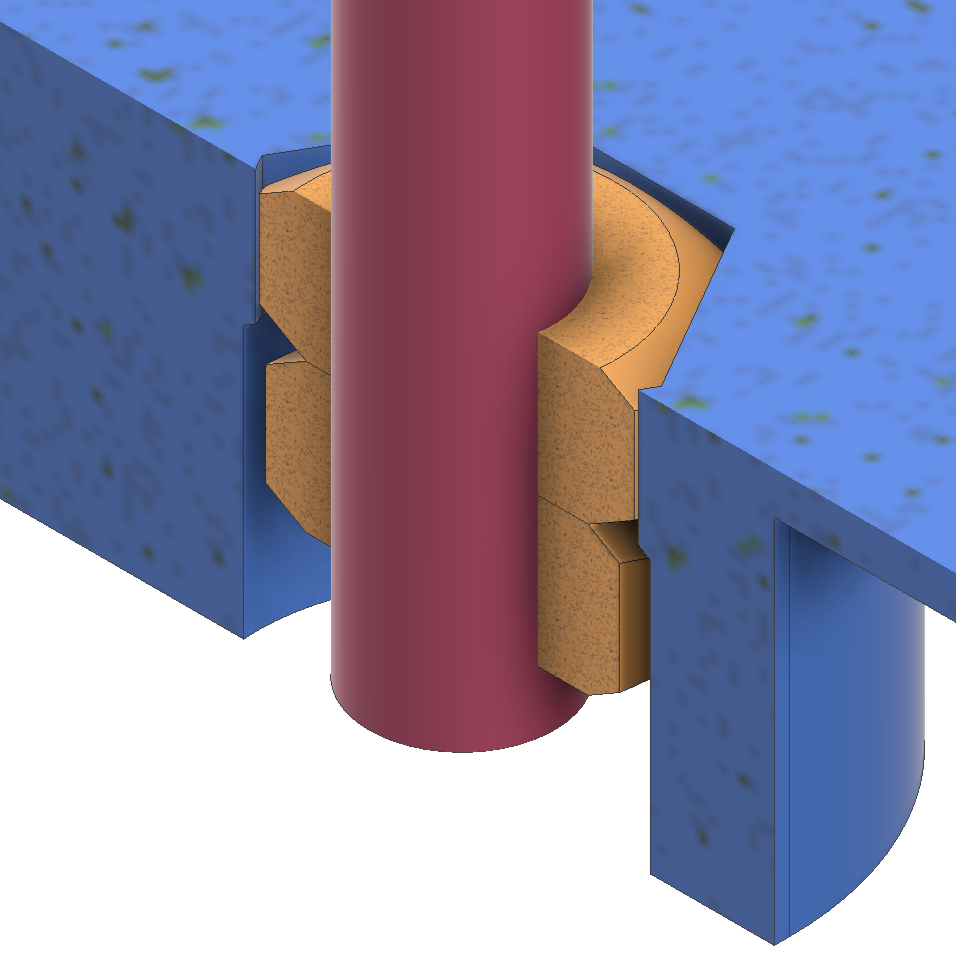
\includegraphics[height=4cm]{figures/InterlockingScrews.png}
        \caption{Tegengedraaide moeren}\label{fig:counterrotated}
    \end{figure}
\end{minipage}\\[12pt]
De bodemplaat is voorzien van verschillende gaten en uitsparingen zoals te zien in. Zo zijn er vier gaten voor de geleidestaven. Ook is er een groot centraal gat voor de loodschroef. Hierin past een lager van formaat ID:4mm, OD:8mm. Verder is er een uitsparing waar een eindeloopschakelaar past. Aan de rand is er een uitsparing waar de spuit in past. Rond deze uitsparing is er een verlaging waar de grepen van de spuit inpassen. Dit alles wordt met een klem vastgehouden doorheen de beweging. Deze klem past in de uitsparing en wordt vastegezet met twee M3 schroeven en de daarvoor voorziene gaten.
\\[12pt]\begin{minipage}[t]{0.49\textwidth}
    \vspace{0pt}
    \begin{figure}[H]
        \centering
        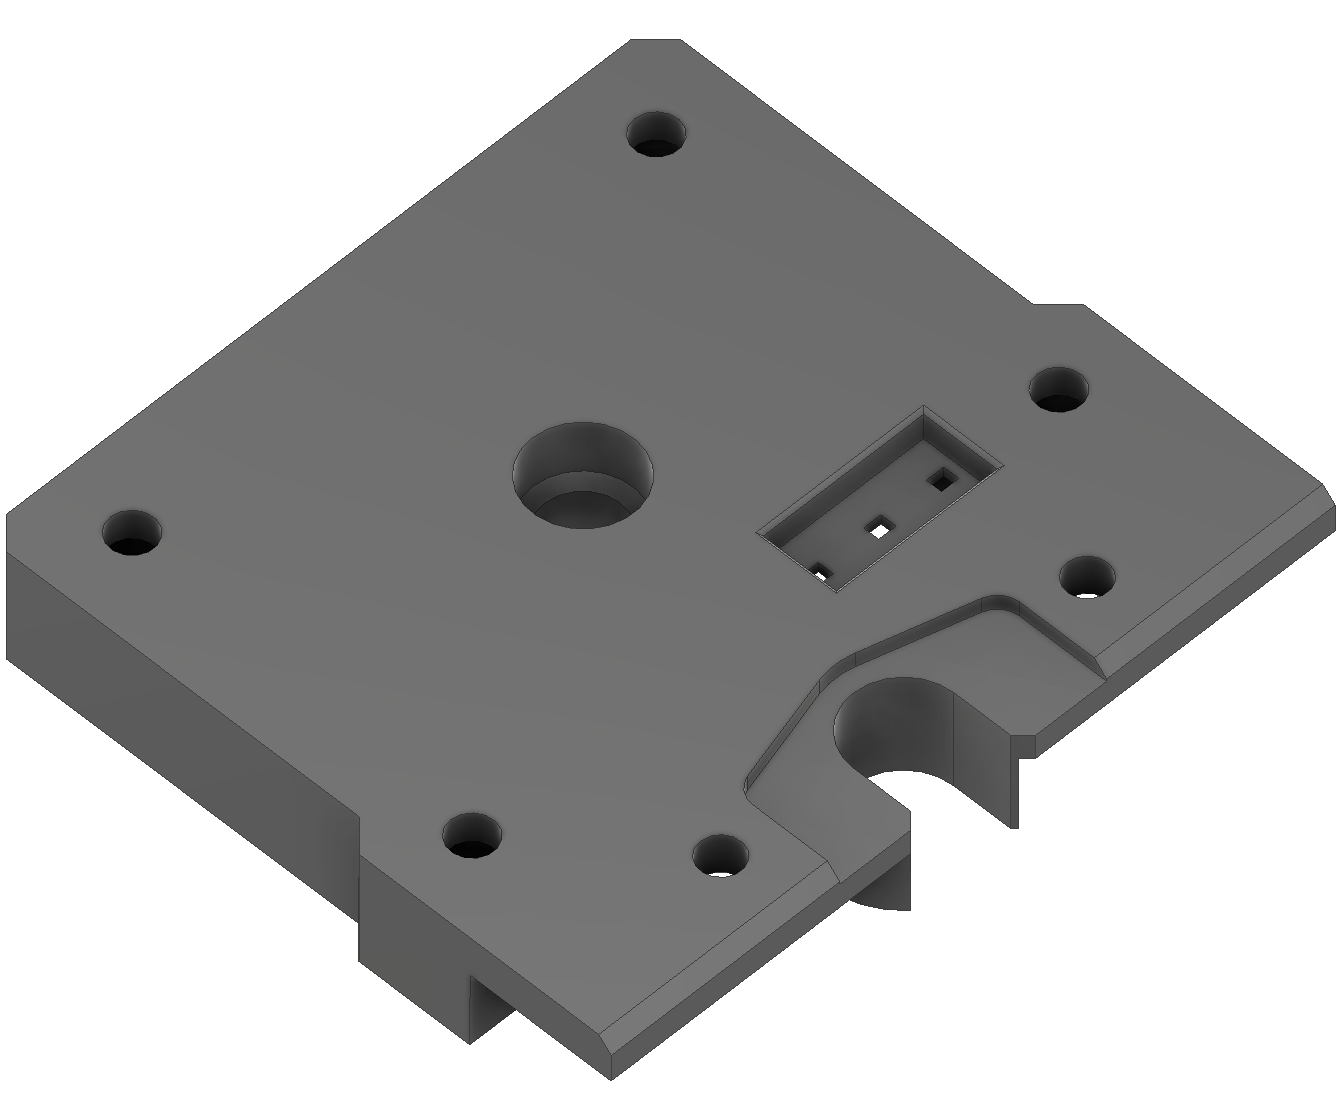
\includegraphics[height=4cm]{figures/Foundation_1_w.png}
        \caption{Bodemplaat.}\label{fig:bodemplaat}
    \end{figure}
\end{minipage}
\begin{minipage}[t]{0.49\textwidth}
    \vspace{0pt}
    \begin{figure}[H]
        \centering
        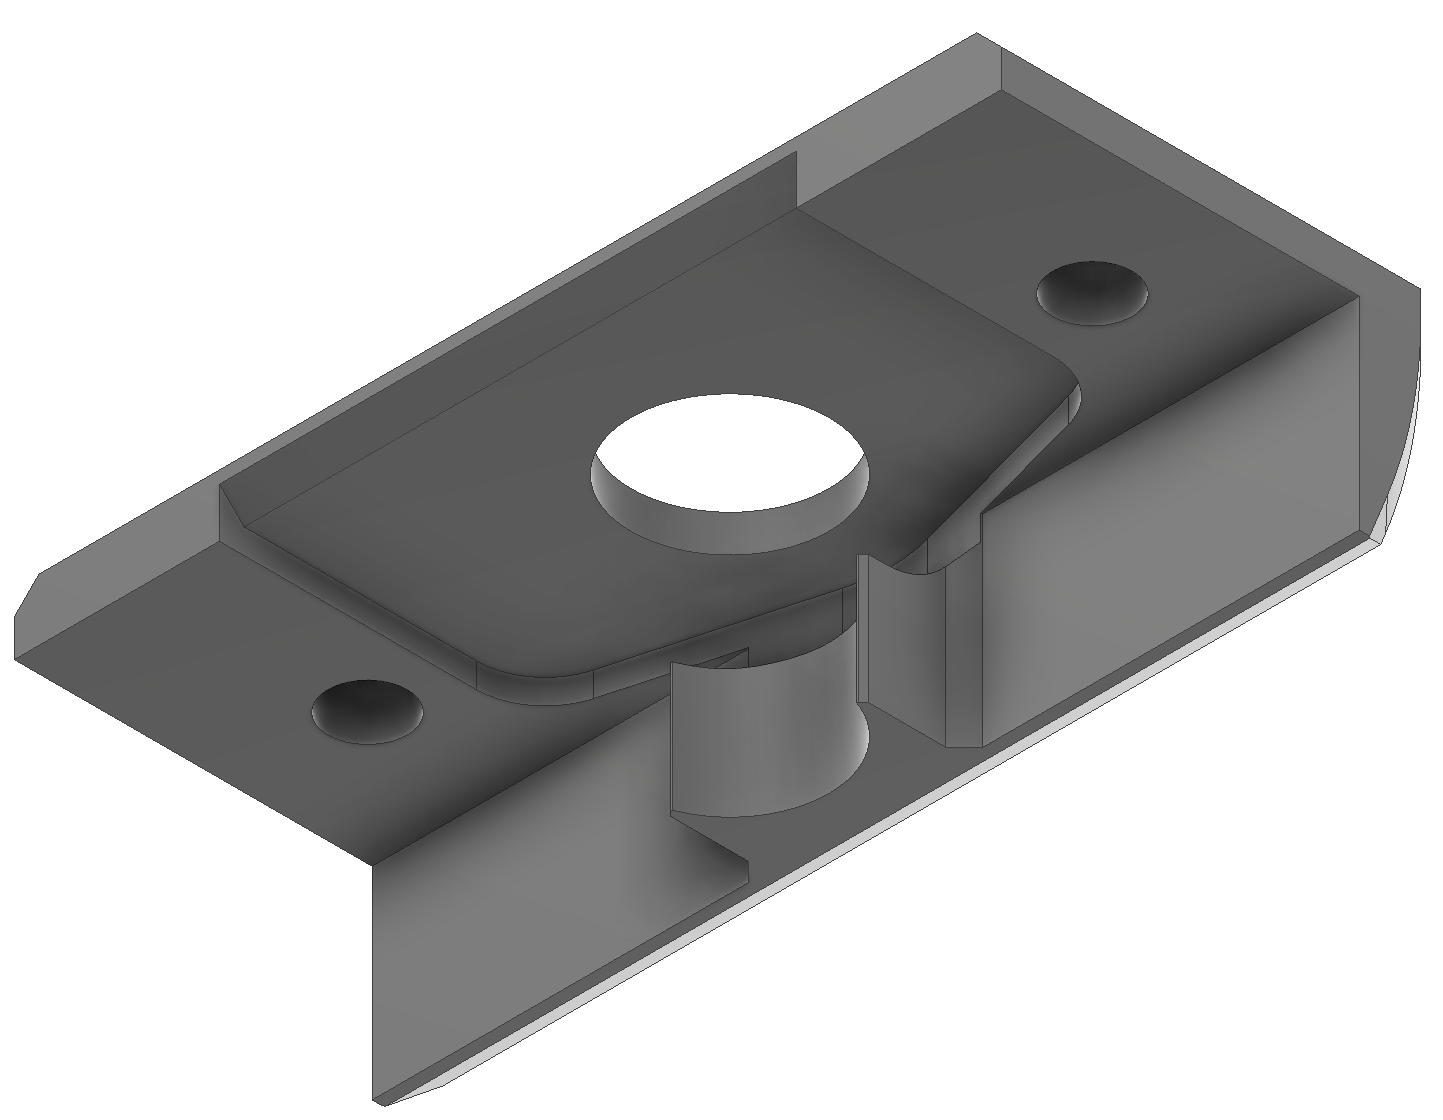
\includegraphics[height=4cm]{figures/Foundation_clamp_w.png}
        \caption{Klem zuiger}\label{fig:clamp}
    \end{figure}
\end{minipage}\\

\subsection{Tussenplaat en motorplaat}
Deze twee platen passen tussen de muurelementen. De tussenplaat vormt de grens tussen de askoppeling en de zuigerkamer. De motorplaat bevindt zich bovenaan en heeft een uitsparing voor een Nema 8 stappermotor die met M2 schroeven bevestigd wordt. 
\\[12pt]\begin{minipage}[t]{0.49\textwidth}
    \vspace{0pt}
    \begin{figure}[H]
        \centering
        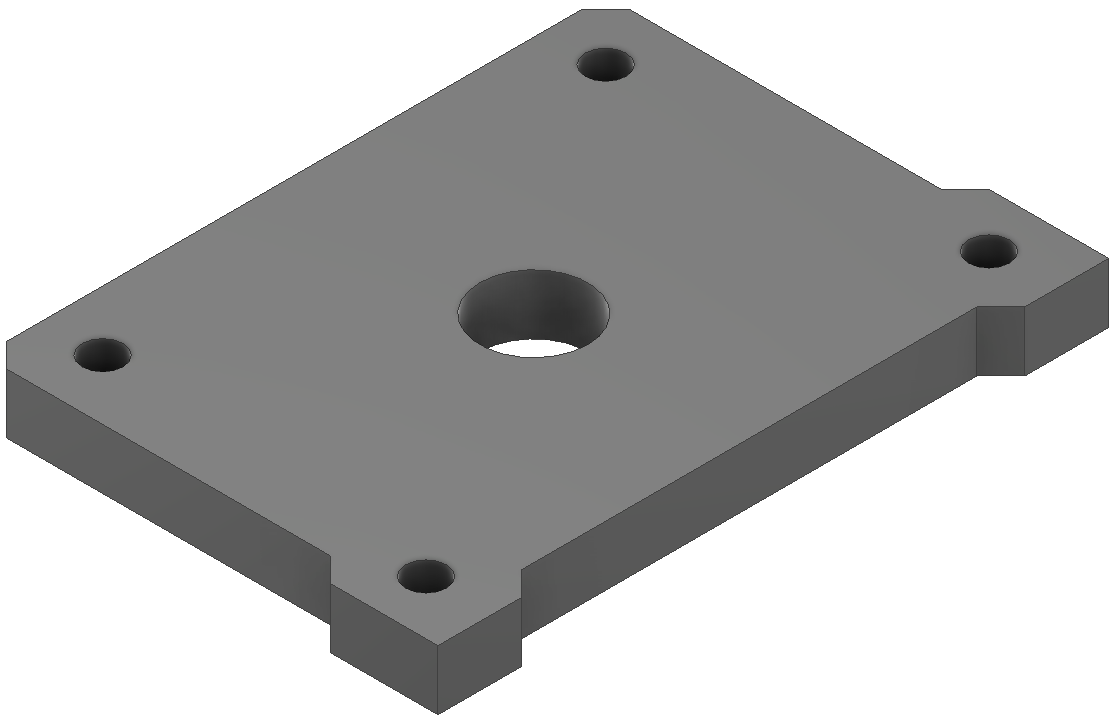
\includegraphics[width=0.65\textwidth]{figures/Topp_Wall_w.png}
        \caption{Tussenplaat.}\label{fig:tussenplaat}
    \end{figure}
\end{minipage}
\begin{minipage}[t]{0.49\textwidth}
    \vspace{0pt}
    \begin{figure}[H]
        \centering
        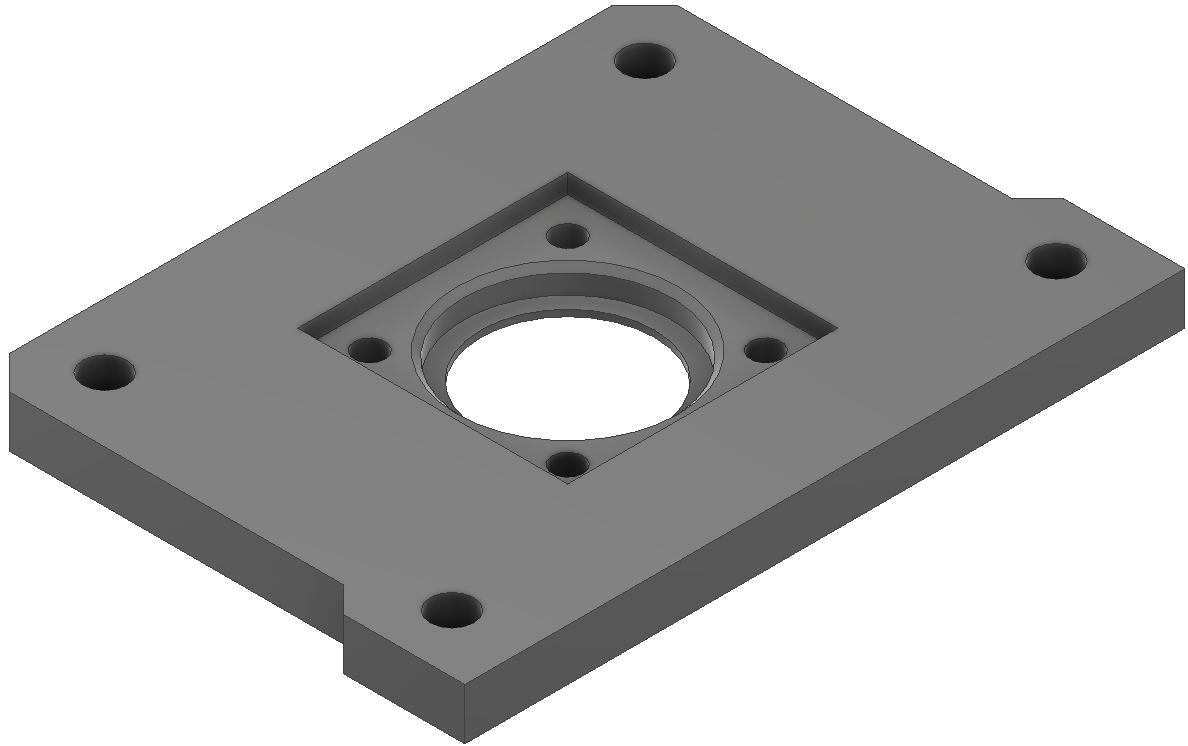
\includegraphics[width=0.65\textwidth]{figures/motor_mount_wide.png}
        \caption{Motorplaat.}\label{fig:motorplaat}
    \end{figure}
\end{minipage}\\

\subsection{Loodschroef, motor en askoppeling}\label{sec: motor}
Voor de loodschroef is een schroef van het type T4 gekozen met een spoed en lood van 1mm. Er is een moer gekozen zonder anti-terugslag mechanische. Terugslag zal namelijk programatisch geëlimineerd worden. De moer heeft 3 gaten, van het formaat M3, die gebruikt worden om de geleideslede te bevestigen.
\\[12pt]De motor is een Nema 8 stappermotor van het type 8HS15--0604D met een maximaal koppel van 0.4N-cm en een stapgrootte van 1.8° per stap. In eerste instantie werd in het ontwerp een zwakkere motor gebruikt (0.2N-cm). Deze mistte echter te veel stappen en is dus vervangen.
\\[12pt]De askoppeling is een flexibele askoppeling van het type 4mm-4mm. Er is gekozen voor een flexibele askoppeling omdat, door het stuikgedrag van PLA na het bevestigen van de moeren, de assen niet meer perfect uitgeliend zijn.

\subsection{Geleideslede}
De geleideslede is het onderdeel dat de zuiger aanstuurt. Deze bestaat uit 3 onderdelen. Het centrale onderdeel, de effectieve slede, is bevestigd met 3 M3 schroeven aan de moer van de loodschroef. Zoals te zien in\ \autoref{fig:CarriageDemonstration} heeft de geleideslede hoge wanden. Deze aanpassing is later in het ontwerp gemaakt toen uit de initiële testen bleek dat de slede de neiging had om to oscilleren. Dit is nu sterk verminderd. Het grotere oppervlak zorgt echter wel voor meer weerstand maar tegenover de zuiger is dit verwaarloosbaar.
\\[12pt]Aan de slede is ook een klem bevestigd. Deze is bevestigd met geleidestaven van 55mm met een bevestiging, gelijkaardig aan die van de grote geleidestaven. De klam bestaat uit twee delen. Het eerste deel heeft een gleuf waar de zuiger in wordt geschoven. De handvaten van de zuiger houden deze op zijn plaats bij de opwaartse slag. Daarna wordt er een bovenste klem bevestigd. Deze klemt de zuiger volledig in. De twee klemmende delen kunnen vervangen worden naargelang de dimensies van de zuiger.
\\[12pt]\begin{minipage}[t]{0.39\textwidth}
    \vspace{0pt}
    \begin{figure}[H]
        \centering
        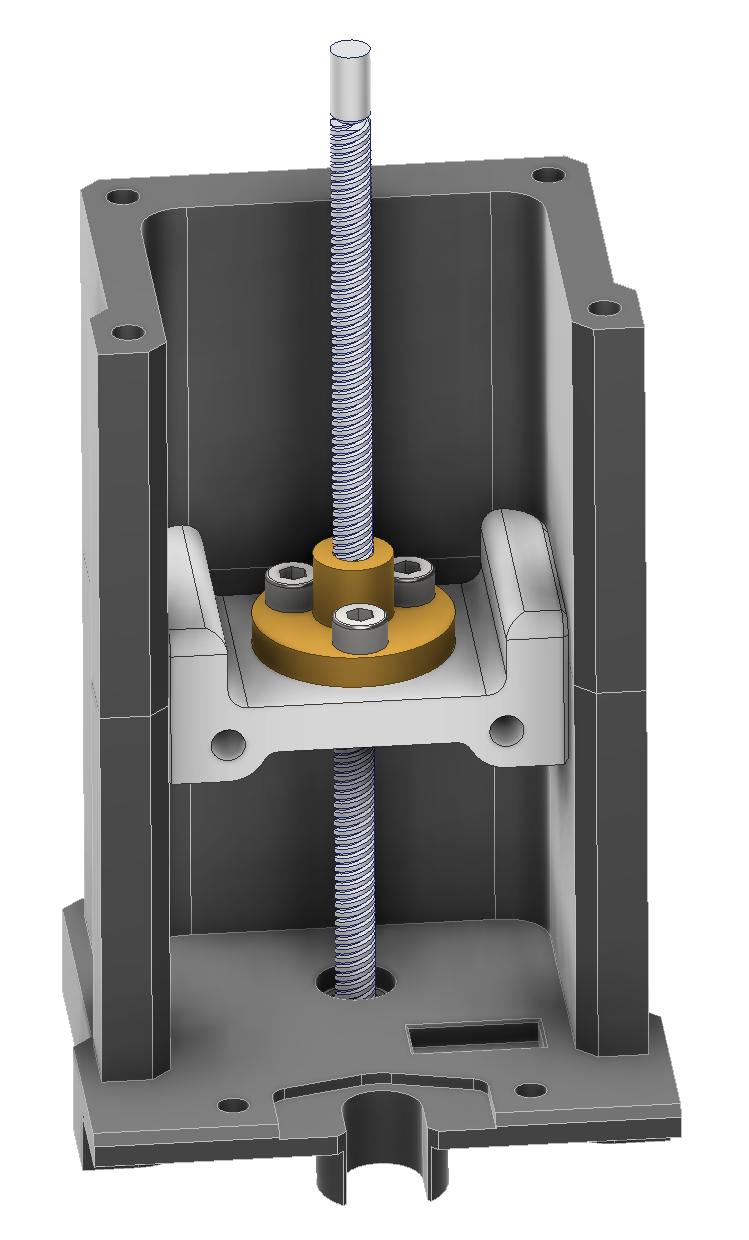
\includegraphics[width=0.65\textwidth]{figures/CarriageDemonstration.png}
        \caption{De geleideslede tussen de muren.}\label{fig:CarriageDemonstration}
    \end{figure}
\end{minipage}
\begin{minipage}[t]{0.59\textwidth}
    \vspace{0pt}
    \begin{figure}[H]
        \centering
        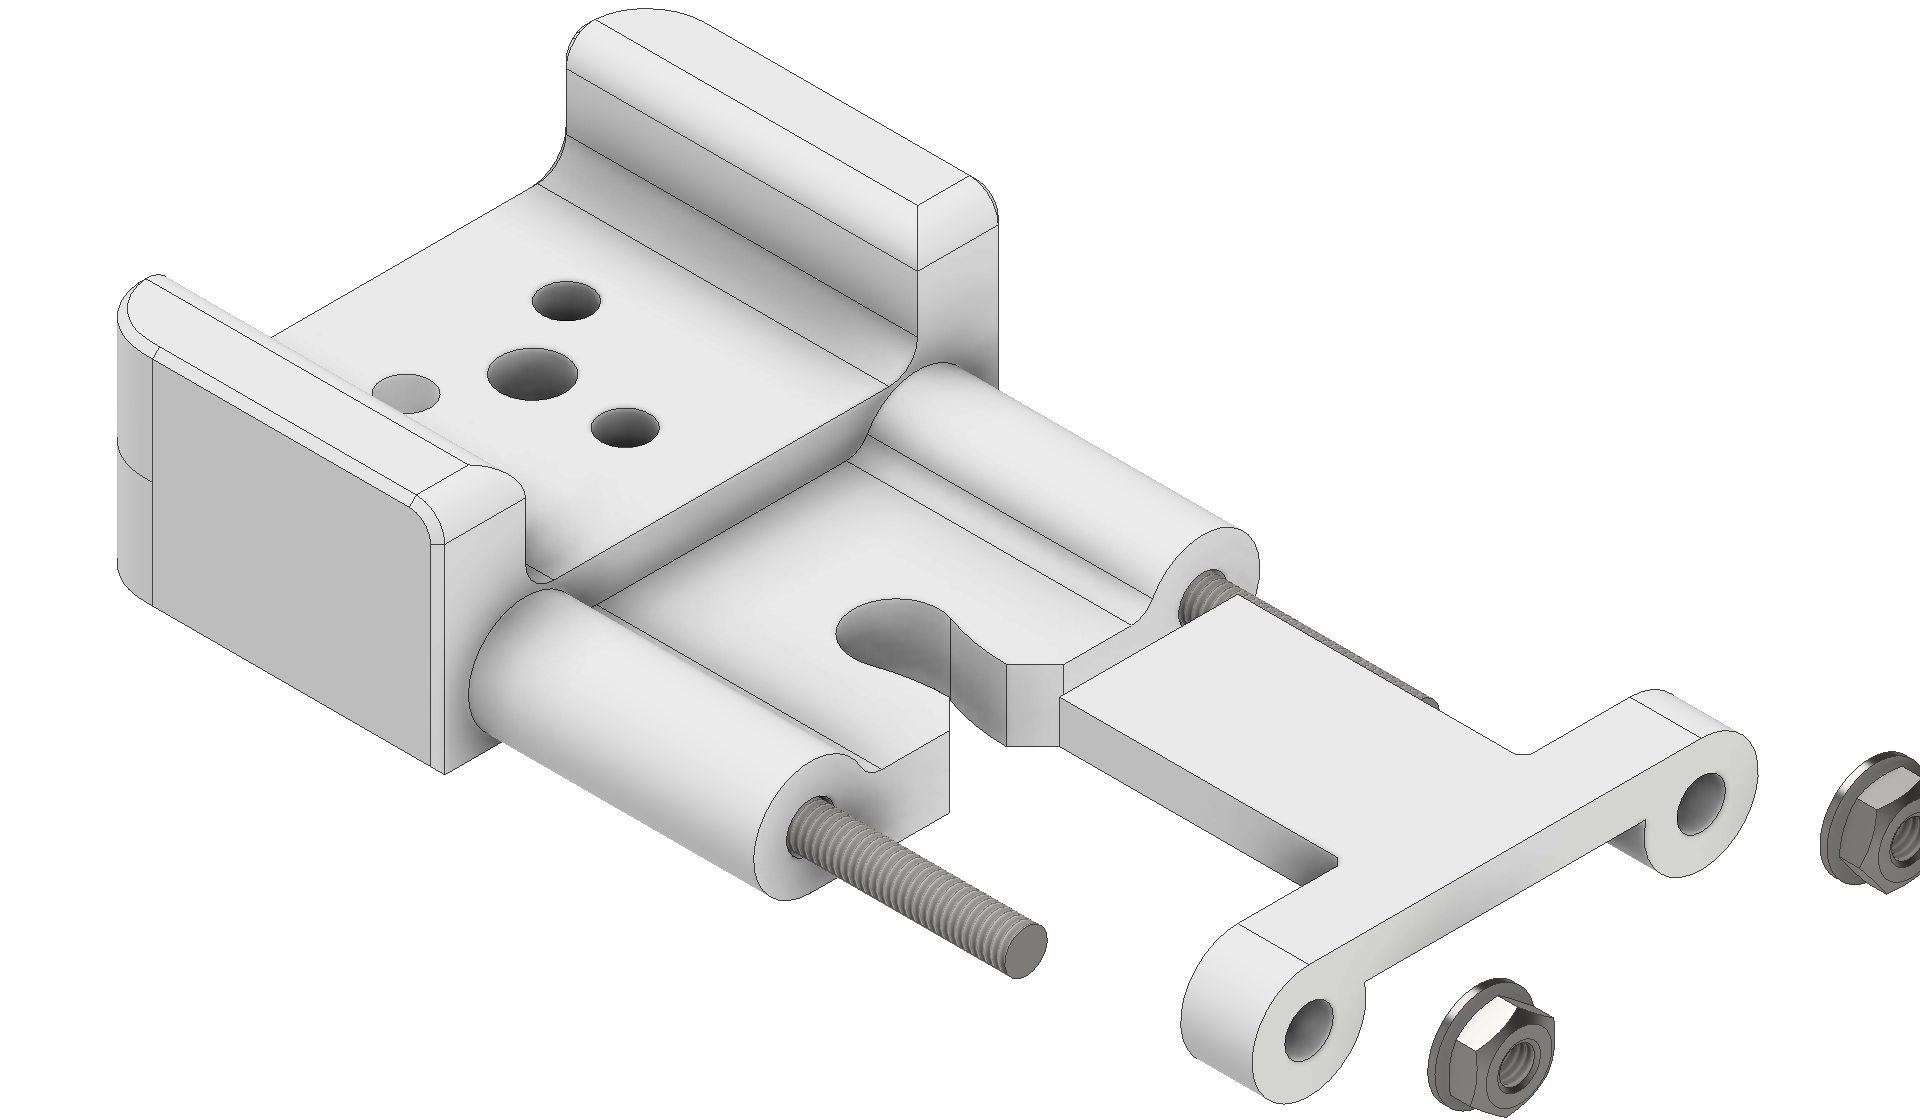
\includegraphics[width=0.85\textwidth]{figures/CarriageAndClamp.png}
        \caption{De geleideslede. Inclusief de samengestelde zuigerklem.}\label{fig:CarriageAndClamp}
    \end{figure}
\end{minipage}\\

\subsection{Zuiger}
Voor de zuiger is gekozen voor standaard verkrijgbare spuiten met een volume van 1000$\mu$l. Deze spuit kan vervangen worden naargelang de gebruikssituatie. In het huidige ontwerp wordt er gewerkt met een spuit van het merk DB, type ISO 7886--1 Luer Slip 1ml. Doordat deze spuiten courant beschikbaar zijn kunnen ze, indien nodig, vervangen worden.
Een belangrijk aspect bij de keuze voor een bestaande spuit was het feit dat ge-3D-print filament niet luchtdicht is en dus geen stabiel vacuum zou kunnen onderhouden. Door een bestaande spuit te gebruiken kan deze bron van fouten deels verholpen worden.

\section{Elektronica ontwerp}
\subsection{Componentenlijst}
\begin{table}[H]
    \begin{tabular}{l|c|c}
        \textbf{Component} & \textbf{Type} & \textbf{Aantal} \\
        \hline
        Motor & Nema 8 (8HS15--0604D)& 1 \\
        Motor driver & BigTreeTech TMC2209 & 1 \\
        Microcontroller & ESP32-WROOM-32 & 1 \\
        eindeloopschakelaar & Micro Limit switch & 1 \\
        5V Voeding & Vrij te kiezen\footnotemark & 1 \\
        \hline
    \end{tabular}
    \caption{Componentenlijst.}\label{tab:componentenlijst}
\end{table}
\footnotetext{{$I_{bron} > 1.7A$}}
\subsection{Motor}
Zoals eerder vermeld in \autoref{sec: motor} is er gekozen voor een Nema 8 motor met een koppel van 0.4N-cm. Dit koppel is voldoende om één zuiger aan te drijven. Een Nema 8 motor is een motor met een relatief klein formaat en past daardoor binnen de afmetingen van het ontwerp. Zoals reeds vernoemd was het ontwerp initieel uitgevoerd met een Nema 8 motor met een koppel van 0.2N-cm. Dit bleek echter te weinig. Deze motor kon de gewenste aspiratiesnelheden niet bereiken en kon de weerstand van de zuiger en geleideslede niet overwinnen.
\\[12pt]De motor heeft 4 aansluitingen (2 per fase) en wordt in dit ontwerp in een open lus gestuurd. Om de fouten te minimaliseren wordt er aangeraden om de pipet zo vaak mogelijk naar de nulpositie te brengen. Hier is een eindeloopschakelaar voor voorzien.
\subsection{Driver}
Er is gekozen voor een TMC2209 stappermotor driver. Deze driver heeft een belangrijk voordeel. Deze kan gebruik maken van zogeheten \"StealthChop\" technologie. Dit zorgt voor een stillere motorwerking. Belangrijk voor deze toepassing is er een soepeler motorverloop met hogere nauwkeurigheid en minder ruis. Een constante pipetteersnelheid is een belangrijke factor in de nauwkeurigheid van de handling. Anderzijds zorgt de het verbeterde stroomprofiel ook voor een verhoging van het effectieve koppel van de motor.\ \cite{RN45}
\subsection{Microcontroller}
Voor de controller is er een ESP32-WROOM-32 gekozen. Deze is voornamelijk gekozen vanwege de hoge kloksnelheid van 80 MHz tot 240 MHz (zie\ \cite{RN46}). Door deze hoge kloksnelheid kan de controller zeer snel stap-signalen naar de driver sturen. Dit is interessant omdat de TMC2209 driver bij kleinere micorstepping een steeds vlotter stroomverloop kan voorzien. Bij micorstepping is de maximale snelheid van de motor echter lager bij een constant aantal stappen/s. Deze stapsnelheid is beperkt door de klok van de controller. De ESP32-WROOM-32 kan de motor dus aan een hoger toerental aandrijven dan meeste andere controllers. Verder is de controller relatief goedkoop (circa €10) en makkelijk te verkrijgen.
\subsection{Aansluiting}
\begin{figure}[H]
    \centering
    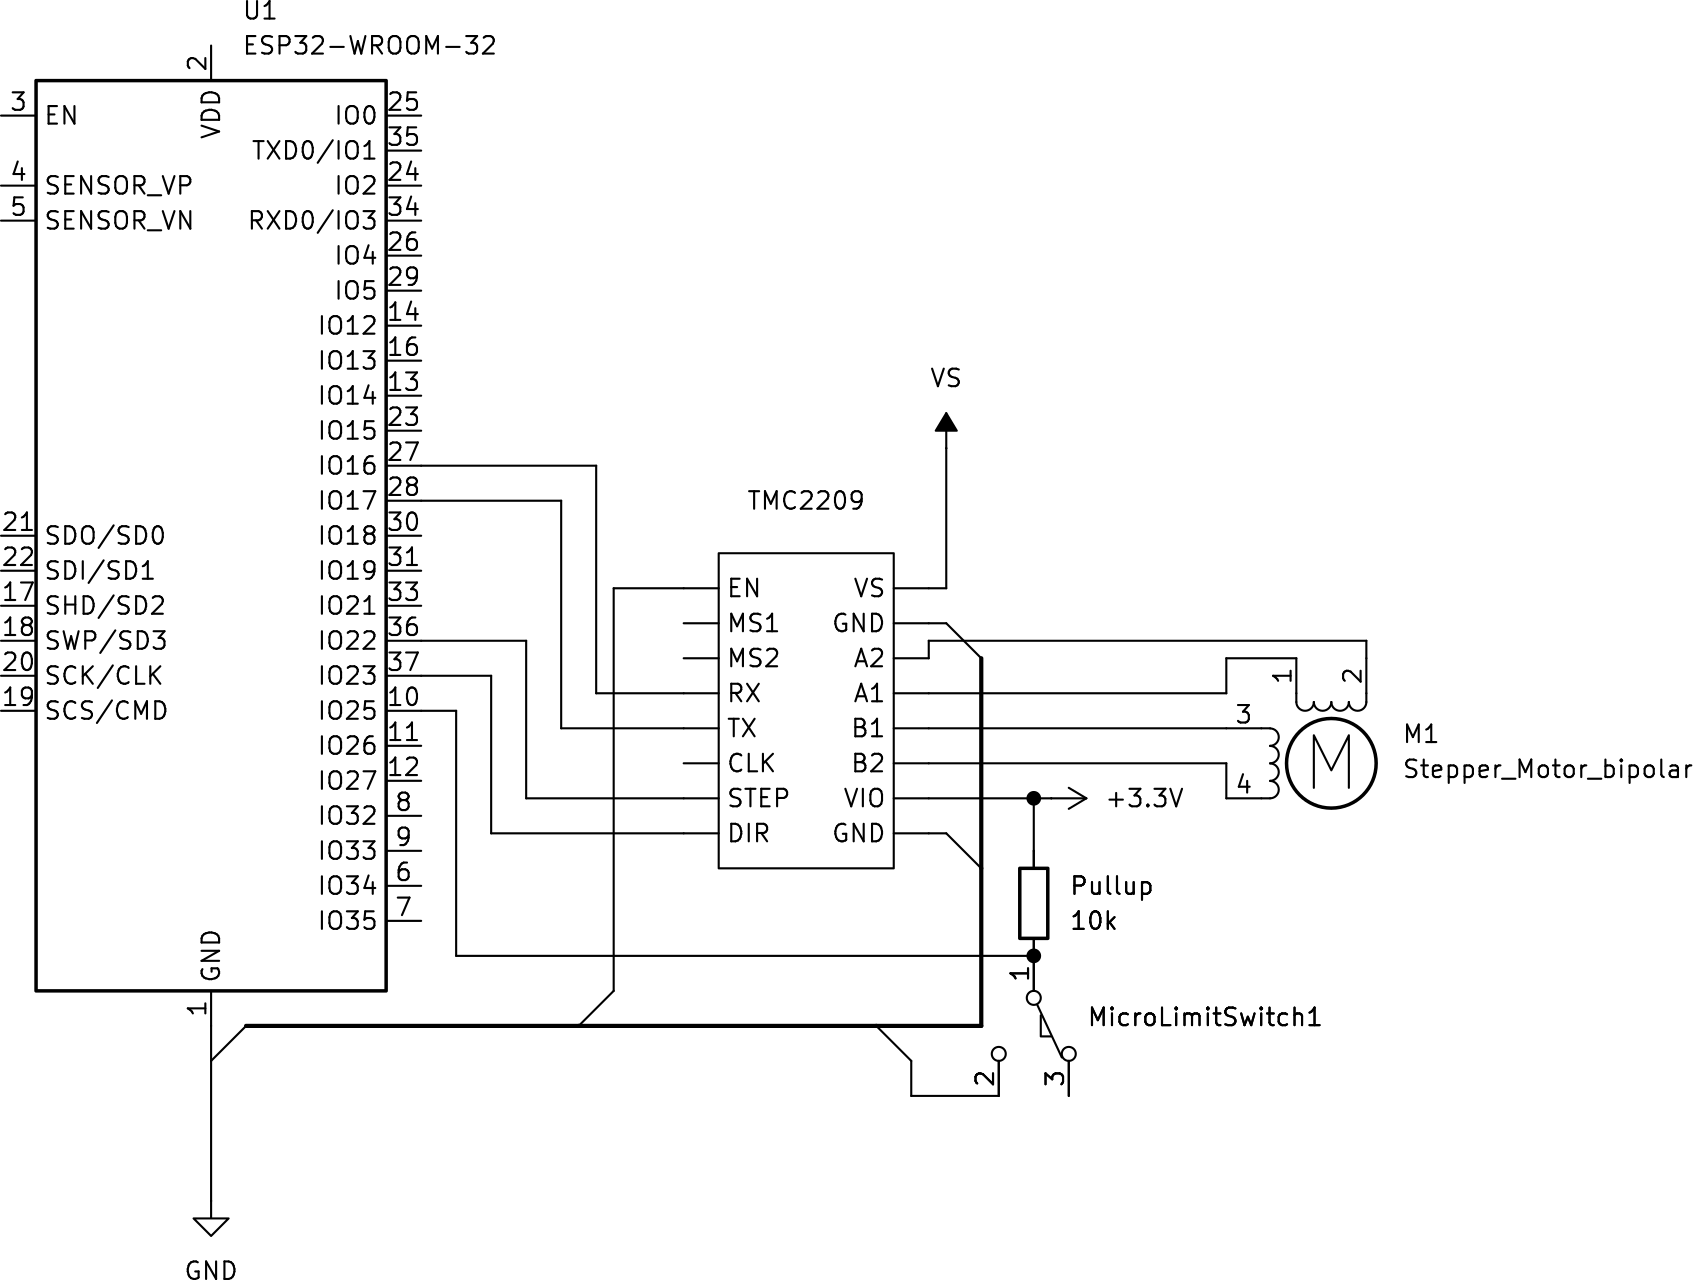
\includegraphics[height=7cm]{figures/Wiring_BW.png}
    \caption{Schema van de aansluiting.}\label{fig:schematische_aansluiting}
\end{figure}

\section{Software ontwerp}


    \chapter{Resultaten}
Voor de ingestelde volumes voldeden alle vier de kanalen aan de ISO 8655 toleranties van maximaal ±4$\mu L$ systematische fout en ±1{,}5$\mu L$ random fout. Bijvoorbeeld, voor een ingesteld volume van 200$\mu L$ waren de gemiddelde volumes respectievelijk 203{,}9$\mu L$, 201{,}5$\mu L$, 201{,}8$\mu L$ en 202{,}8$\mu L$, met systematische fouten tussen 1{,}5 en 3{,}9$\mu L$ en random fouten onder 1{,}3$\mu L$, zie ook Tabel\ref{tab:accuracies}.

\begin{table}[H] \centering \begin{tabular}{c|c|c|c} 
    \textbf{Gewenste Volume} & \textbf{Gemiddelde ($\mu L$)} & \textbf{Systematische fout ($\mu L$)} & \textbf{Random fout ($\mu L$)}\\
    \hline
    100 & 99.9 & –0.1 & 0.67 \\
    200 & 203.9 & 3.9 & 0.51 \\ 
    300 & 000 & 000 & 000 \\
    400 & 000 & 000 & 000 \\
    500 & 000 & 000 & 000 \\
    600 & 000 & 000 & 000 \\
    700 & 000 & 000 & 000 \\
    800 & 000 & 000 & 000 \\
    900 & 000 & 000 & 000 \\
    1000 & 000 & 000 & 000 \\   

\end{tabular} \caption{Resultaten van nauwkeurigheidstesten per kanaal (n=10).}\label{tab:accuracies} \end{table}

Deze resultaten tonen aan dat het systeem voldoet aan de eisen van ISO 8655 voor zowel precisie als nauwkeurigheid, en dus geschikt is voor gebruik in laboratoriumomgevingen met hoge kwaliteitseisen
Hierbij wordt het voorbeeld gevolgd van\ \cite{RN49}. Hier wordt ook een spuit-gebaseerd ontwerp getest op nauwkeurigheid met een beschreven procedure.
    \chapter{Conclusies}
In deze bachelorproef werd een modulair, kostenefficiënt pipetteersysteem ontworpen en gerealiseerd met het oog op het verbeteren van reproduceerbaarheid in laboratoria. De opzet was om een systeem te ontwikkelen dat als end effector kan functioneren binnen een groter geautomatiseerd laboratorium, met specifieke toepassing binnen de onderzoeksgroep \textit{Translational Neurosciences} aan de Universiteit Antwerpen.
\\[12pt]Door een combinatie van 3D-geprinte componenten, een nauwkeurig aangedreven lineaire beweging via een loodschroef, en een aanstuurbare microcontroller werd een robuust systeem gerealiseerd. De resultaten van de nauwkeurigheidstesten toonden aan dat de pipet voldoet aan de ISO 8655 normen, wat de geschiktheid van dit ontwerp voor laboratoriumgebruik bevestigt.
\\[12pt]Samenvattend kan worden gesteld dat de ontwerp- en implementatievereisten succesvol zijn ingevuld. Dit pipettesysteem biedt een waardevol alternatief voor dure commerciële oplossingen, met behoud van precisie, reproduceerbaarheid en gebruiksgemak.
\\[12pt]\textbf{Aanbevelingen voor toekomstig werk} zijn onder andere:
\begin{itemize}
  \item Integratie van closed-loop feedback om gemiste stappen te detecteren.
  \item Ontwikkeling van een multi-channel versie voor hoger throughput.
  \item Validatie in een reële laboratoriumsetting met biologische monsters.
\end{itemize}
    \input{chapters/06_reflection}


    

    
    % -------------------------------------------------------------------
    % Bibliography/References  -  Harvard Style was used in this report
    % -------------------------------------------------------------------
    \bibliography{references_truncated.bib}  %  Patashnik, O. (1988), BibTEXing. Documentation for general BibTEX users.
    
    % -------------------------------------------------------------------
    % Appendices
    % -------------------------------------------------------------------
    
    \begin{appendices}
        \chapter{}
\section{Metingen}
\subsection{Metingen spuit 1}
\begin{itemize}
    \item Luchtdruk: 102,1 kPa
    \item Temperatuur: 22,0 °C
    \item Correctiefactor Z:\ 1,0033 (zie\ \cite{RN50})
\end{itemize}
\begin{table}[H] 
    \centering 
    \caption{Resultaten van nauwkeurigheidstesten van de opstelling spuit 1}
    \begin{tabular}{|c|c|c|c|}
        \hline
        \textbf{\rule{0pt}{3ex} Gewenste Volume [$\mu L$]} & 100 & 500 & 1000 \\
        \hline
        \textbf{Metingen [$\mu L$]} & 99,6 & 501,2 & 1001,9\\
        &100,0 & 500,8 & 1001,5\\
        &98,8 & 500,9 & 998,7\\
        &100,2 & 499,8 & 999,1\\
        &99,8 & 500,0 & 998,8\\
        &100,6 & 502,3 & 1000,8\\
        &100,5 & 501,1 & 1000,4\\
        &98,9 & 500,1 & 999,0\\
        &100,4 & 500,2 & 999,1\\
        &100,0 & 502,9 & 998,7\\
        \hline
        \textbf{Gemiddelde [$\mu L$]} & 100,2 & 502,6 & 1003,1\\
        \textbf{Systematische fout [\%]} & 0,21 & 0,52 & 0,31\\
        \textbf{Willekeurige fout [\%]} & 0,63 & 0,20 & 0,12\\
        \hline
    \end{tabular}\label{tab:resultaten_spuit_1}
\end{table}

\pagebreak

\subsection{Metingen spuit 2}
\begin{itemize}
    \item Luchtdruk: 000 kPa
    \item Temperatuur: 000 °C
    \item Correctiefactor Z:\ 000 (zie\ \cite{RN50})
\end{itemize}
\begin{table}[H] 
    \centering 
    \caption{Resultaten van nauwkeurigheidstesten van de opstelling spuit 2}
    \begin{tabular}{|c|c|c|c|}
        \hline
        \textbf{\rule{0pt}{3ex} Gewenste Volume [$\mu L$]} & 100 & 500 & 1000 \\
        \hline
        \textbf{Metingen [$\mu L$]}& 000 & 000 & 000\\
        &000 & 000 & 000\\
        &000 & 000 & 000\\
        &000 & 000 & 000\\
        &000 & 000 & 000\\
        &000 & 000 & 000\\
        &000 & 000 & 000\\
        &000 & 000 & 000\\
        &000 & 000 & 000\\
        &000 & 000 & 000\\
        \hline
        \textbf{Gemiddelde [$\mu L$]} &000 & 000 & 000\\
        \textbf{Systematische fout [\%]} &000 & 000 & 000\\
        \textbf{Willekeurige fout [\%]} &000 & 000 & 000\\
        \hline
    \end{tabular}\label{tab:resultaten_spuit_2}
\end{table}
        \input{chapters/appendix_B.tex}
    \end{appendices}
    
\end{document}
